\documentclass[../text/main.tex]{subfiles}


\begin{document}

\section{Supplementary Figures}
\label{supp-figures}


\begin{sifigure}[H]
	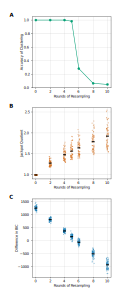
\includegraphics[width=0.619\textwidth]{jackpotting.pdf}
	\caption{\textbf{Jackpotting causes false clusters.} (Continued on next page.)}
	\label{jackpotting}
\end{sifigure}
\addtocounter{sifigure}{-1}
\pagebreak
\begin{sifigure}[H]
	\caption[]{(Continued from previous page.) \textbf{(A)} The fraction of 60 FASTQ files (each of a random 280~nt RNA with 1 structure and 200,000 simulated reads) for which SEISMIC-RNA correctly found 1 cluster as a function of the number of rounds of resampling 200,000 reads with replacement. \textbf{(B)} The distribution of jackpotting quotients for each number of rounds of resampling. Horizontal black bars show means. \textbf{(C)} The distribution of the difference in BIC between 2 clusters and 1 cluster for each number of rounds of resampling. Horizontal black bars show means.}
\end{sifigure}
\pagebreak


\begin{sifigure}[H]
	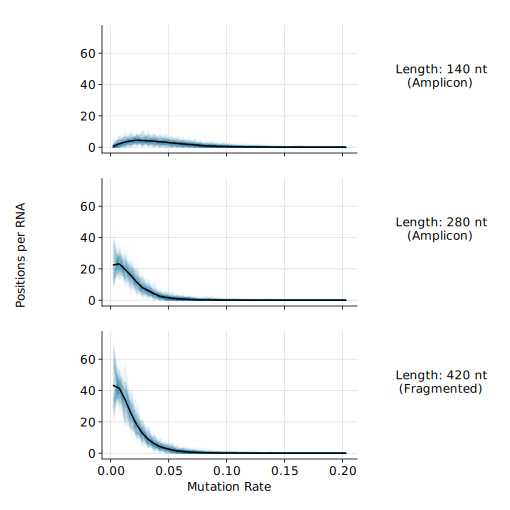
\includegraphics[width=\textwidth]{mus-hist-200000.pdf}
	\caption{\textbf{Histogram of mutation rates using 200,000 reads.} For each reference length, the histogram of the mutation rates on A and C positions for all 240 RNAs with 200,000 simulated reads (transparent blue). The black line shows the average. The bin size for the histogram is 0.005.}
    \label{mus-hist-200000}
\end{sifigure}
\pagebreak


\begin{sifigure}[H]
	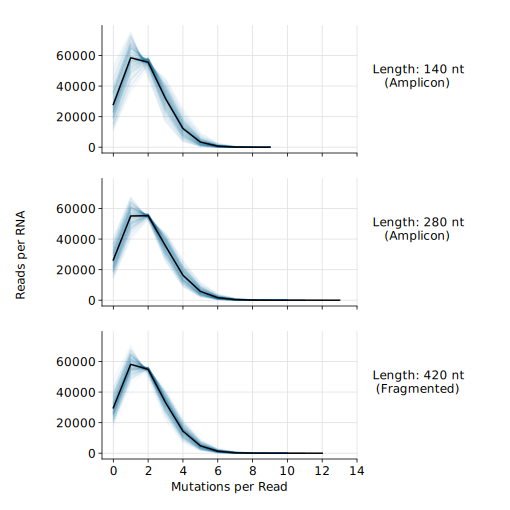
\includegraphics[width=\textwidth]{nmut-hist-200000.pdf}
	\caption{\textbf{Histogram of number of mutated bases per read using 200,000 reads.} For each reference length, the histogram of the number of mutated bases for all 240 RNAs with 200,000 simulated reads (transparent blue). The black line shows the average. The RNAs were simulated to have an average of 2 mutations per read.}
	\label{nmut-hist-200000}
\end{sifigure}
\pagebreak


\begin{sifigure}[H]
	\includegraphics[width=\textwidth]{ncov-200000.pdf}
	\caption{\textbf{Read coverage per position using 200,000 reads.} For each reference length, the number of informative base calls at each position for all 240 RNAs with 200,000 simulated reads (transparent blue). The black line shows the average.}
	\label{ncov-200000}
\end{sifigure}
\pagebreak


\begin{sifigure}[H]
	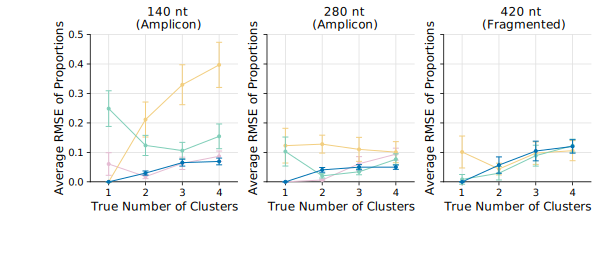
\includegraphics[width=\textwidth]{average-pis-rmse_main-200000.pdf}
	\caption{\textbf{Accuracy of cluster proportions using 200,000 reads.} Average root-mean-square error (RMSE) between the true cluster proportions and those calculated by SEISMIC-RNA, DanceMapper, DRACO, and DREEM for each length of RNA and true number of clusters. Lower RMSEs are more accurate. Error bars show 95\% confidence intervals.}
	\label{average-pis-rmse_main-200000}
\end{sifigure}
\pagebreak


\begin{sifigure}[H]
	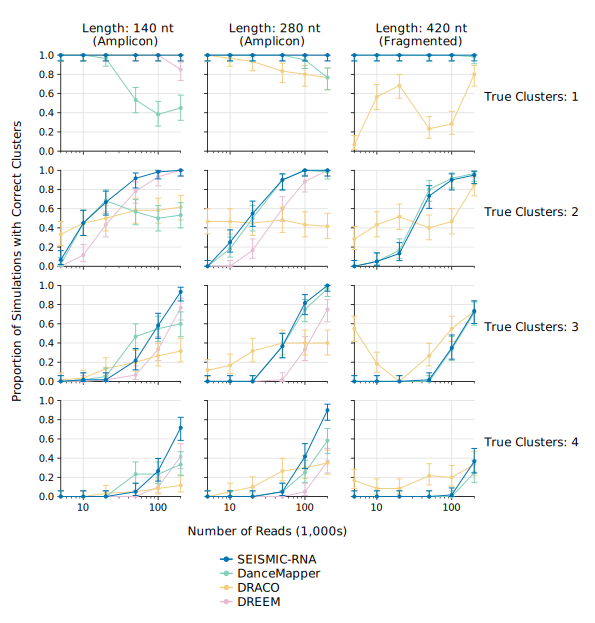
\includegraphics[width=\textwidth]{vs-reads-correct-k-main.pdf}
	\caption{\textbf{Accuracy of number of clusters versus number of reads for each software.} Proportion of simulated FASTQ files for which each piece of software detected the correct number of clusters as a function of number of reads for each reference length and true number of clusters. Higher proportions are more accurate. Error bars show 95\% confidence intervals.}
	\label{vs-reads-correct-k-main}
\end{sifigure}
\pagebreak


\begin{sifigure}[H]
	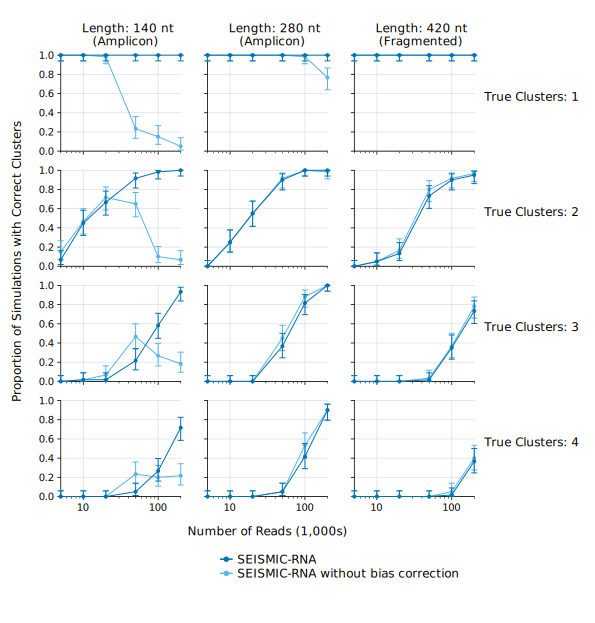
\includegraphics[width=\textwidth]{vs-reads-correct-k-seismic.pdf}
	\caption{\textbf{Accuracy of number of clusters versus number of reads without bias correction.} Proportion of simulated FASTQ files for which SEISMIC-RNA with and without bias correction detected the correct number of clusters as a function of number of reads for each reference length and true number of clusters. Higher proportions are more accurate. Error bars show 95\% confidence intervals.}
	\label{vs-reads-correct-k-seismic}
\end{sifigure}
\pagebreak


\begin{sifigure}[H]
	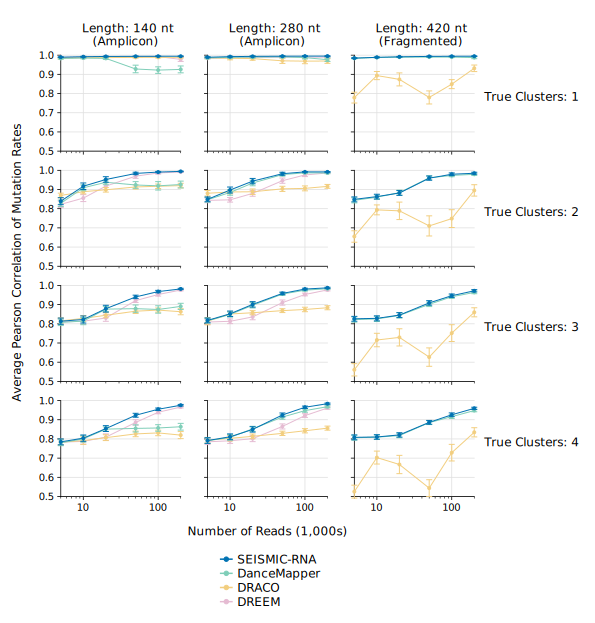
\includegraphics[width=\textwidth]{vs-reads-mus-pcc-main.pdf}
	\caption{\textbf{Accuracy of mutation rates versus number of reads for each software.} Average Pearson correlation between the true mutation rates and the mutation rates detected by each piece of software as a function of number of reads for each reference length and true number of clusters. Higher correlations are more accurate. Error bars show 95\% confidence intervals.}
	\label{vs-reads-mus-pcc-main}
\end{sifigure}
\pagebreak


\begin{sifigure}[H]
	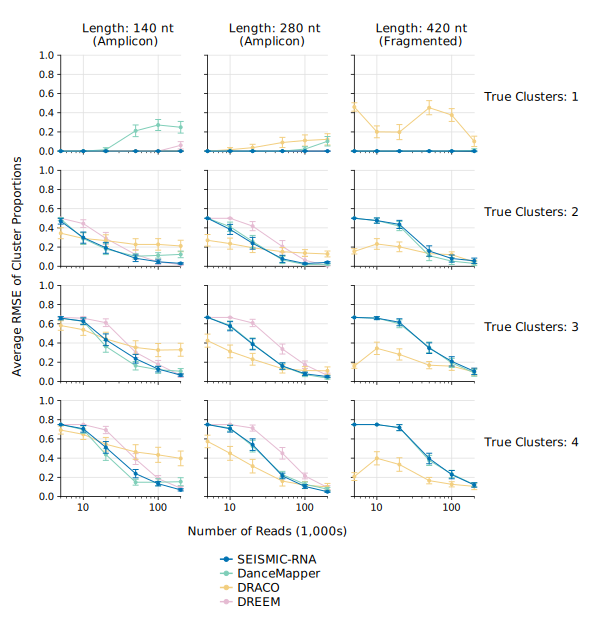
\includegraphics[width=\textwidth]{vs-reads-pis-rmse-main.pdf}
	\caption{\textbf{Accuracy of cluster proportions versus number of reads for each software.} Average root-mean-square error (RMSE) between the true cluster proportions and the cluster proportions detected by each piece of software as a function of number of reads for each reference length and true number of clusters. Lower RMSEs are more accurate. Error bars show 95\% confidence intervals.}
	\label{vs-reads-pis-rmse-main}
\end{sifigure}
\pagebreak


\begin{sifigure}[H]
	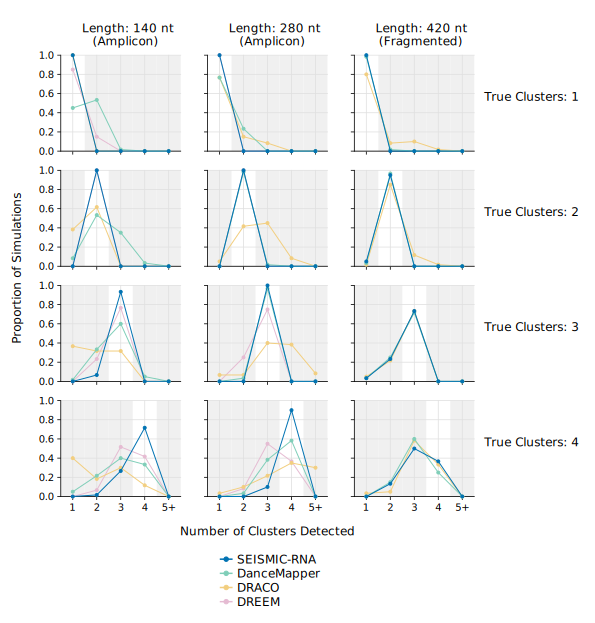
\includegraphics[width=\textwidth]{proportion-each-k-main-200000.pdf}
	\caption{\textbf{Distribution of number of clusters detected using 200,000 reads.} Proportion of simulated FASTQ files for which each piece of software detected each number of clusters for each reference length and true number of clusters.}
	\label{proportion-each-k-main-200000}
\end{sifigure}
\pagebreak


\begin{sifigure}[H]
	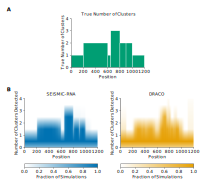
\includegraphics[width=\textwidth]{long-transcript-ks.pdf}
	\caption{\textbf{Number of clusters detected at each position in long transcripts.} \textbf{(A)} Location, length, and number of clusters formed by each ground truth domain in every 1,200~nt RNA. Domains are surrounded by white borders to help distinguish them visually. \textbf{(B)} Fraction of 60 simulated 1,200~nt RNAs for which SEISMIC-RNA and DRACO detected each number of clusters at each position. Cluster numbers are cumulative: e.g. if at position 1, 25\% of RNAs yielded 1 cluster, 50\% yielded 2, and 25\% yielded 3, then the area between 2 and 3 on the y axis (meaning at least 3 clusters) would be 25\% dark, between 1 and 2 (meaning at least 2 clusters) would be 75\% dark, and between 0 and 1 (meaning at least 1 cluster) would be 100\% dark.}
	\label{long-transcript-ks}
\end{sifigure}
\pagebreak


\begin{sifigure}[H]
	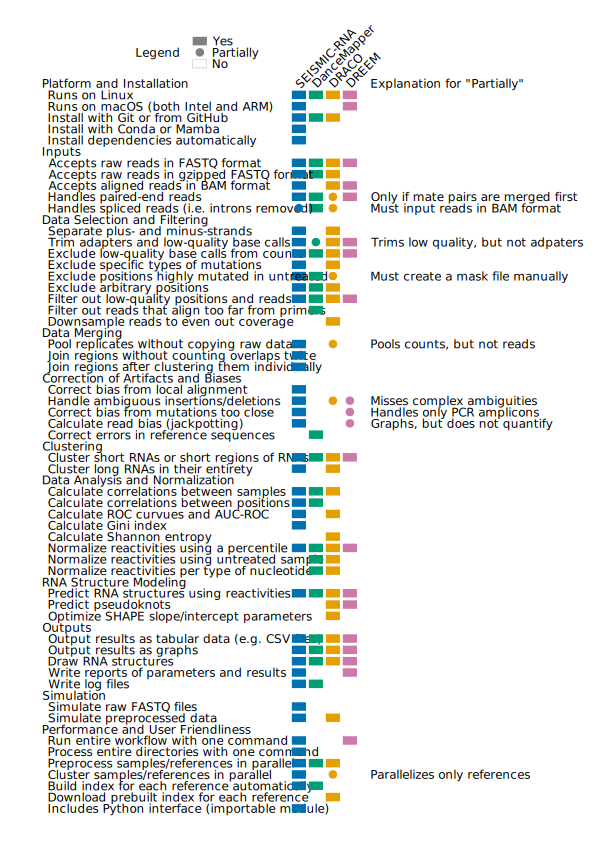
\includegraphics[width=\textwidth]{features.pdf}
	\caption{\textbf{SEISMIC-RNA offers unique features compared to other software.} (Continued on next page.)}
	\label{features}
\end{sifigure}
\addtocounter{sifigure}{-1}
\pagebreak
\begin{sifigure}[H]
	\caption[]{(Continued from previous page.) A list of features supported by each piece of software. For DanceMapper~\cite{Olson2022} and DRACO~\cite{Morandi2021}, this chart includes the features of ShapeMapper~2~\cite{Busan2018} and RNA Framework~\cite{Incarnato2018}, respectively, which are required for preprocessing the data before clustering. For each feature that is ``Partially" supported, an explanation of what specifically is supported is given in the right column.}
\end{sifigure}
\pagebreak


\end{document}
